\documentclass[aspectratio=169,10pt]{beamer}

% -----------------------------------------------------------------------------
% Sparse FFN project presentation - native LaTeX Beamer source
% Theme: Deep Teal / Mint / Coral (distinct from the navy-gold reference deck)
% Compile: pdflatex Sparse_FFN_Beamer_Presentation.tex (twice)
% -----------------------------------------------------------------------------

\usetheme{default}
\usefonttheme{professionalfonts}
\usepackage[T1]{fontenc}
\usepackage{lmodern}
\usepackage{amsmath,amssymb,mathtools,bm}
\usepackage{graphicx}
\usepackage{booktabs,tabularx,array,multirow}
\usepackage{ragged2e}
\usepackage{tikz}
\usetikzlibrary{positioning,arrows.meta,calc,shapes.geometric,fit}
\usepackage{hyperref}
\usepackage{microtype}
\usepackage{siunitx}
\sisetup{detect-all,group-separator={,},group-minimum-digits=4}

% --- Colour palette ---
\definecolor{DeepTeal}{HTML}{09353B}
\definecolor{ForestTeal}{HTML}{087A78}
\definecolor{Mint}{HTML}{56C7B2}
\definecolor{Coral}{HTML}{E76F51}
\definecolor{WarmAmber}{HTML}{F2B45B}
\definecolor{Paper}{HTML}{F5F8F7}
\definecolor{TealTint}{HTML}{E7F4F1}
\definecolor{CoralTint}{HTML}{FCEEEA}
\definecolor{Slate}{HTML}{263B40}
\definecolor{Muted}{HTML}{62757A}
\definecolor{LineGray}{HTML}{D6E0DD}

\setbeamercolor{normal text}{fg=Slate,bg=white}
\setbeamercolor{structure}{fg=ForestTeal}
\setbeamercolor{frametitle}{fg=white,bg=DeepTeal}
\setbeamercolor{title}{fg=white}
\setbeamercolor{subtitle}{fg=Mint}
\setbeamercolor{block title}{fg=white,bg=ForestTeal}
\setbeamercolor{block body}{fg=Slate,bg=TealTint}
\setbeamercolor{alertblock title}{fg=white,bg=Coral}
\setbeamercolor{alertblock body}{fg=Slate,bg=CoralTint}
\setbeamercolor{exampleblock title}{fg=white,bg=DeepTeal}
\setbeamercolor{exampleblock body}{fg=Slate,bg=Paper}
\setbeamercolor{itemize item}{fg=Coral}
\setbeamercolor{itemize subitem}{fg=ForestTeal}
\setbeamercolor{footline}{fg=white,bg=DeepTeal}
\setbeamercolor{takeaway}{fg=white,bg=DeepTeal}

\setbeamerfont{title}{size=\LARGE,series=\bfseries}
\setbeamerfont{subtitle}{size=\large}
\setbeamerfont{frametitle}{size=\large,series=\bfseries}
\setbeamerfont{block title}{series=\bfseries}
\setbeamertemplate{navigation symbols}{}
\setbeamertemplate{itemize item}{\raise0.15ex\hbox{\scriptsize\color{Coral}$\blacktriangleright$}}
\setbeamertemplate{itemize subitem}{\raise0.1ex\hbox{\tiny\color{ForestTeal}$\blacktriangleright$}}
\setbeamertemplate{enumerate item}{\color{ForestTeal}\insertenumlabel.}

% Header and footer
\setbeamertemplate{frametitle}{%
  \nointerlineskip%
  \begin{beamercolorbox}[wd=\paperwidth,ht=0.67cm,dp=0.16cm,leftskip=0.46cm,rightskip=0.42cm]{frametitle}%
    \usebeamerfont{frametitle}\insertframetitle%
    \hfill{\color{Mint}\scriptsize\insertsection}%
  \end{beamercolorbox}%
}
\setbeamertemplate{footline}{%
  \leavevmode%
  \hbox{%
    \begin{beamercolorbox}[wd=.74\paperwidth,ht=2.6ex,dp=1.05ex,leftskip=.45cm]{footline}%
      \scriptsize\color{white}Sparse FFN | NIT Mizoram \hspace{1em}\textcolor{Mint}{\textbullet}\hspace{.45em} Multivariate Statistical Analysis
    \end{beamercolorbox}%
    \begin{beamercolorbox}[wd=.26\paperwidth,ht=2.6ex,dp=1.05ex,rightskip=.45cm plus1fil]{footline}%
      \scriptsize\color{white}\hfill\insertframenumber\,/\,\inserttotalframenumber
    \end{beamercolorbox}%
  }%
}

\setbeamersize{text margin left=0.52cm,text margin right=0.52cm}
\setlength{\abovedisplayskip}{4pt}
\setlength{\belowdisplayskip}{4pt}
\setlength{\abovedisplayshortskip}{2pt}
\setlength{\belowdisplayshortskip}{2pt}
\renewcommand{\arraystretch}{1.12}

% Helper components
\newcommand{\metricbox}[3]{%
  \begin{beamercolorbox}[wd=\linewidth,rounded=true,sep=5pt,center]{block body}%
    {\color{ForestTeal}\Large\bfseries #1}\par\vspace{1pt}
    {\footnotesize\bfseries #2}\par
    {\scriptsize\color{Muted}#3}
  \end{beamercolorbox}%
}
\newcommand{\takeaway}[1]{%
  \begin{beamercolorbox}[wd=\linewidth,rounded=true,sep=6pt]{takeaway}%
    {\small\bfseries\color{Mint}KEY TAKEAWAY}\par\vspace{2pt}{\small #1}
  \end{beamercolorbox}%
}
\newcommand{\rqbadge}[1]{\tikz[baseline=(x.base)]\node[rounded corners=2pt,fill=Coral,text=white,inner xsep=5pt,inner ysep=2pt,font=\bfseries\scriptsize](x){#1};}
\newcommand{\smallnote}[1]{{\scriptsize\color{Muted}#1}}
\newcommand{\Hnull}{\mathcal{H}_0}
\newcommand{\erank}{\operatorname{erank}}
\newcommand{\PR}{\operatorname{PR}}
\newcommand{\ReLU}{\operatorname{ReLU}}
\newcommand{\I}{\mathbb{I}}
\newcommand{\R}{\mathbb{R}}
\newcommand{\E}{\mathbf{E}}
\newcommand{\Var}{\operatorname{Var}}

\title{Statistical Characterisation of Sparse Activations and Low-Rank Latent Structures in Dense Feed-Forward Neural Networks}
\subtitle{A multivariate statistical study of OPT-125M on WikiText-2}
\author{Lakshmi Ganapathi Kodi (BT23MA005) \and Saurabh Kumar Gupta (BT23MA006)}
\institute{Department of Mathematics\\National Institute of Technology Mizoram\\[2pt]Under the guidance of Prof. Ashis SenGupta\\Applied Statistics Unit, Indian Statistical Institute, Kolkata}
\date{November 2026}

\begin{document}

% -----------------------------------------------------------------------------
% 1. Title
% -----------------------------------------------------------------------------
\begin{frame}[plain]
\begin{tikzpicture}[remember picture,overlay]
  \fill[DeepTeal] (current page.north west) rectangle ([yshift=-3.45cm]current page.north east);
  \fill[ForestTeal] ([yshift=-3.45cm]current page.north west) rectangle ([yshift=-3.57cm]current page.north east);
  \fill[Mint] ([xshift=-1.3cm,yshift=-3.45cm]current page.north east) -- ([xshift=-.7cm,yshift=-3.45cm]current page.north east) -- ([xshift=-1.3cm,yshift=-3.57cm]current page.north east) -- cycle;
  \fill[Coral] ([xshift=0.35cm,yshift=0.35cm]current page.south west) circle (0.12cm);
  \fill[WarmAmber] ([xshift=0.72cm,yshift=0.35cm]current page.south west) circle (0.12cm);
\end{tikzpicture}
\vspace{0.35cm}
{\color{Mint}\small CSP 1602  |  MULTIVARIATE STATISTICAL ANALYSIS}\par
\vspace{0.55cm}
{\color{white}\large\bfseries Statistical Characterisation of Sparse Activations and Low-Rank Latent Structures in Dense Feed-Forward Neural Networks}\par
\vspace{0.22cm}
{\color{Mint}\normalsize Layer dynamics, neuron dependence, intrinsic dimensionality and domain sensitivity}\par
\vspace{1.1cm}
\begin{center}
{\large\bfseries Lakshmi Ganapathi Kodi}\quad {\small(BT23MA005)}\\[3pt]
{\large\bfseries Saurabh Kumar Gupta}\quad {\small(BT23MA006)}\\[0.7cm]
{\small Under the guidance of}\par
{\large\bfseries Prof. Ashis SenGupta}\par
{\small Applied Statistics Unit, Indian Statistical Institute, Kolkata}\par
\vspace{0.45cm}
{\small Department of Mathematics}\par
{\small National Institute of Technology Mizoram}\par
{\small November 2026}
\end{center}
\end{frame}

% -----------------------------------------------------------------------------
% 2. Roadmap
% -----------------------------------------------------------------------------
\section{Overview}
\begin{frame}{Presentation Roadmap}
\begin{columns}[T,onlytextwidth]
\column{.48\textwidth}
\begin{block}{FOUNDATION}
\begin{enumerate}
  \item Motivation and problem statement
  \item Project objectives and hypotheses
  \item Model, dataset and activation pipeline
\end{enumerate}
\end{block}
\begin{block}{STATISTICAL FORMULATION}
\begin{enumerate}\setcounter{enumi}{3}
  \item RQ1: Layer-wise sparsity profile
  \item RQ2: Neuron co-activation
  \item RQ3: Latent dimensionality
\end{enumerate}
\end{block}
\column{.48\textwidth}
\begin{block}{EMPIRICAL EVIDENCE}
\begin{enumerate}\setcounter{enumi}{6}
  \item RQ4: Weights versus activations
  \item RQ5: Cross-domain representations
  \item Integrated findings and implications
\end{enumerate}
\end{block}
\begin{alertblock}{FINAL DISCUSSION}
Conclusion, limitations, future work and questions.
\end{alertblock}
\end{columns}
\end{frame}

% -----------------------------------------------------------------------------
% 3. Motivation
% -----------------------------------------------------------------------------
\begin{frame}{Motivation: The Dense-Weight / Sparse-Activation Paradox}
\begin{columns}[T,onlytextwidth]
\column{.56\textwidth}
\begin{block}{Why focus on Transformer FFNs?}
\begin{itemize}
  \item FFN sub-layers contain a large share of the parameters and computation in Transformer blocks.
  \item In OPT-125M, a token representation expands from 768 to 3,072 dimensions.
  \item ReLU sets every negative pre-activation to an exact zero.
  \item The weight matrices remain dense even when most intermediate neurons are inactive for a token.
\end{itemize}
\end{block}
\takeaway{The project asks how much of the nominal 3,072-dimensional FFN space is actually used, how that use changes with depth, and what structure is present in the active features.}
\column{.40\textwidth}
\metricbox{768}{Model width $d_{model}$}{Input token representation}
\vspace{5pt}
\metricbox{3,072}{FFN width $d_{ffn}$}{Intermediate feature space}
\vspace{5pt}
\metricbox{12}{Transformer layers}{OPT-125M decoder stack}
\end{columns}
\end{frame}

% -----------------------------------------------------------------------------
% 4. Model equation and research questions
% -----------------------------------------------------------------------------
\begin{frame}{FFN Computation and Five Research Questions}
\begin{block}{Feed-forward computation in each Transformer layer}
\[
  \mathbf{h}^{(\ell)}=\ReLU\!\left(\mathbf{x}^{(\ell)}\mathbf{W}_1^{(\ell)}+\mathbf{b}_1^{(\ell)}\right),
  \qquad
  \mathbf{y}^{(\ell)}=\mathbf{h}^{(\ell)}\mathbf{W}_2^{(\ell)}+\mathbf{b}_2^{(\ell)}.
\]
\end{block}
\small
\begin{tabularx}{\linewidth}{>{\bfseries}p{0.08\linewidth} X X}
\toprule
RQ & Research question & Null hypothesis (summary)\\
\midrule
RQ1 & Is sparsity constant across the 12 layers? & $\mu_0=\mu_1=\cdots=\mu_{11}$\\
RQ2 & Do neurons co-activate or fire independently? & $\phi_{ij}=0$ for all $i\ne j$\\
RQ3 & Is the activation space full-dimensional? & $\erank(\mathbf{S})=3,072$\\
RQ4 & Do weight and activation ranks track each other? & Static and dynamic ranks are directly coupled\\
RQ5 & Are activation manifolds invariant across text domains? & $\boldsymbol\mu_{wiki}=\boldsymbol\mu_{sci}=\boldsymbol\mu_{news}$\\
\bottomrule
\end{tabularx}
\vspace{4pt}
\smallnote{These hypotheses organise the analyses; individual test assumptions and estimands are described on the corresponding RQ slides.}
\end{frame}

% -----------------------------------------------------------------------------
% 5. Pipeline
% -----------------------------------------------------------------------------
\begin{frame}{Experimental Architecture: From Text to Statistical Evidence}
\centering
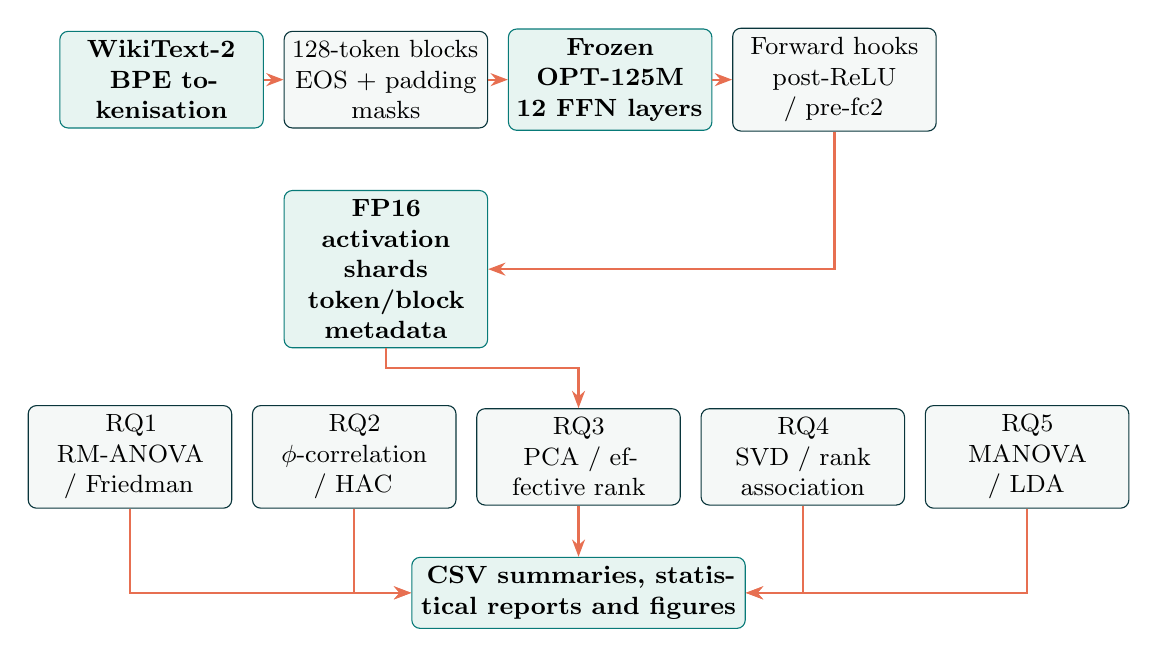
\begin{tikzpicture}[
  node distance=0.42cm and 0.25cm,
  stage/.style={rounded corners=3pt,draw=ForestTeal,fill=TealTint,minimum height=0.86cm,text width=2.35cm,align=center,font=\small\bfseries},
  proc/.style={rounded corners=3pt,draw=DeepTeal,fill=Paper,minimum height=0.86cm,text width=2.35cm,align=center,font=\small},
  arr/.style={-{Stealth[length=2.2mm]},thick,color=Coral}
]
\node[stage] (data) {WikiText-2\\BPE tokenisation};
\node[proc,right=of data] (chunks) {128-token blocks\\EOS + padding masks};
\node[stage,right=of chunks] (model) {Frozen OPT-125M\\12 FFN layers};
\node[proc,right=of model] (hooks) {Forward hooks\\post-ReLU / pre-fc2};
\draw[arr] (data)--(chunks); \draw[arr] (chunks)--(model); \draw[arr] (model)--(hooks);
\node[stage,below=0.78cm of chunks] (store) {FP16 activation shards\\token/block metadata};
\draw[arr] (hooks.south) |- (store.east);
\node[proc,below=0.72cm of store,xshift=-3.25cm] (rq1) {RQ1\\RM-ANOVA / Friedman};
\node[proc,right=0.25cm of rq1] (rq2) {RQ2\\$\phi$-correlation / HAC};
\node[proc,right=0.25cm of rq2] (rq3) {RQ3\\PCA / effective rank};
\node[proc,right=0.25cm of rq3] (rq4) {RQ4\\SVD / rank association};
\node[proc,right=0.25cm of rq4] (rq5) {RQ5\\MANOVA / LDA};
\draw[arr] (store.south) -- ++(0,-0.25) -| (rq3.north);
\node[stage,below=0.65cm of rq3,text width=4.0cm] (out) {CSV summaries, statistical reports and figures};
\draw[arr] (rq1.south) |- (out.west);
\draw[arr] (rq2.south) |- (out.west);
\draw[arr] (rq3.south) -- (out.north);
\draw[arr] (rq4.south) |- (out.east);
\draw[arr] (rq5.south) |- (out.east);
\end{tikzpicture}
\end{frame}

% -----------------------------------------------------------------------------
% 6. Dataset / extraction
% -----------------------------------------------------------------------------
\begin{frame}{Dataset and Activation Extraction}
\begin{columns}[T,onlytextwidth]
\column{.5\textwidth}
\begin{block}{Text processing}
\begin{itemize}
  \item Primary corpus: Salesforce WikiText-2 raw-v1.
  \item OPT-125M byte-pair encoding tokenizer.
  \item End-of-sequence marker preserved between source rows.
  \item Non-overlapping contiguous blocks of length $L=128$.
  \item Padding positions are tracked and excluded from summaries.
\end{itemize}
\end{block}
\column{.47\textwidth}
\begin{block}{Activation capture}
\[
\mathbf{H}^{(\ell)}=\ReLU\!\left(\operatorname{fc1}^{(\ell)}(\mathbf{X}^{(\ell)})\right)
\in\R^{B\times L\times 3072}.
\]
\begin{itemize}
  \item Twelve decoder-layer activation hooks.
  \item Captured post-ReLU and before the second FFN projection.
  \item Non-padding tokens retained; values stored as FP16 shards.
  \item Token positions and block IDs retained for block-level inference.
\end{itemize}
\end{block}
\end{columns}
\vspace{2pt}
\smallnote{Sampling discipline: for RQ1, independent 128-token text blocks are the repeated-measures units, not individual neighbouring tokens.}
\end{frame}

% -----------------------------------------------------------------------------
% 7. Basic statistical setup
% -----------------------------------------------------------------------------
\begin{frame}{Mathematical Setup: Sparsity as a Layer-wise Profile}
Let $h_{t,k}^{(\ell)}$ be the post-ReLU activation of neuron $k$ for token $t$ in layer $\ell$.
\begin{block}{Token-wise activation sparsity}
\[
  s_t^{(\ell)}=\frac{1}{d_{ffn}}\sum_{k=1}^{d_{ffn}}\I\!\left(h_{t,k}^{(\ell)}=0\right),
  \qquad d_{ffn}=3072.
\]
\end{block}
\begin{block}{Block-averaged profile used for RQ1}
For independent text block $B_i$ and layer $\ell$:
\[
  s_{i\ell}=\frac{1}{|B_i|d_{ffn}}
  \sum_{t\in B_i}\sum_{k=1}^{d_{ffn}}\I\!\left(h_{t,k}^{(\ell)}=0\right).
\]
\end{block}
\vspace{2pt}
\small\textbf{Interpretation:} If $s=0.90$, around 10\% of intermediate neurons are active. At $s=0.9877$, only about 38 of 3,072 neurons are active.
\end{frame}

% -----------------------------------------------------------------------------
% 8. RQ1 method
% -----------------------------------------------------------------------------
\section{Research Questions}
\begin{frame}{RQ1 | Target and Statistical Formulation}
\rqbadge{RQ1}\quad\textbf{Layer-wise sparsity non-flatness}
\begin{block}{Target and null hypothesis}
Test whether the mean block-level sparsity profile is flat across all 12 FFN layers:
\[
  \Hnull:\mu_0=\mu_1=\cdots=\mu_{11}
  \qquad\text{versus}\qquad
  H_A:\text{at least one layer mean differs.}
\]
\end{block}
\small
\begin{columns}[T,onlytextwidth]
\column{.49\textwidth}
\begin{block}{Contrast Hotelling's $T^2$}
\[
T^2=n(C\bar{\mathbf{s}})^T
\left(C\mathbf{S}C^T\right)^{-1}
(C\bar{\mathbf{s}}),
\]
\small where $C$ encodes layer contrasts.
\end{block}
\column{.49\textwidth}
\begin{block}{Repeated-measures ANOVA}
\[
F=\frac{MS_{\mathrm{layer}}}{MS_{\mathrm{error}}},
\qquad \widehat\epsilon_{GG}\in\left[\frac{1}{p-1},1\right].
\]
\small Greenhouse--Geisser adjusts degrees of freedom when sphericity fails.
\end{block}
\end{columns}
\vspace{2pt}
\small\textbf{Friedman rank test:}\quad
$Q=\dfrac{12}{np(p+1)}\sum_{j=1}^{p}R_j^2-3n(p+1)$, with $p=12$ layers.
\end{frame}

% -----------------------------------------------------------------------------
% 9. RQ1 results
% -----------------------------------------------------------------------------
\begin{frame}{RQ1 | Evidence: A Sharp Sparsity Peak at Layer 3}
\begin{columns}[T,onlytextwidth]
\column{.60\textwidth}
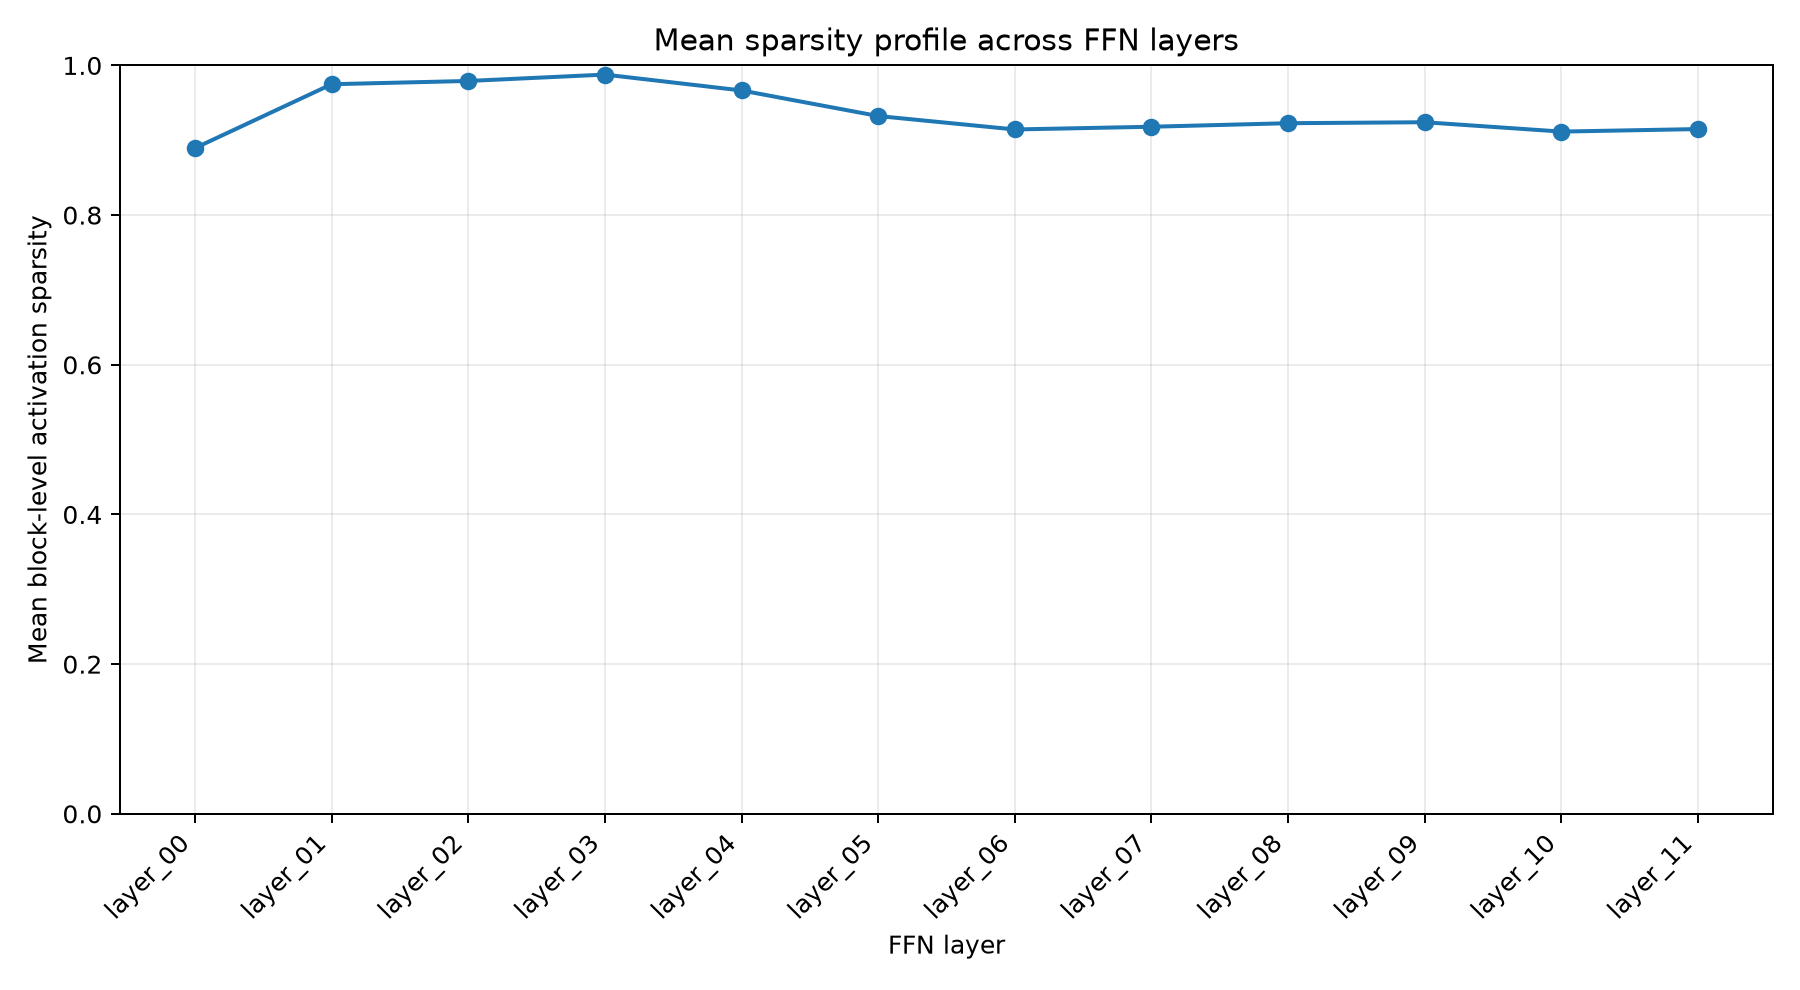
\includegraphics[width=\linewidth,height=4.3cm,keepaspectratio]{assets/rq1_layer_sparsity.png}
\column{.38\textwidth}
\begin{block}{Layer-wise profile}
\small
\textbf{L0:} 88.96\% sparse (about 339 active neurons).\par\vspace{4pt}
\textbf{L3:} 98.77\% sparse (about 38 active neurons).\par\vspace{4pt}
\textbf{L6--L11:} 91.16--92.41\% sparse. L5 is 93.23\%.
\end{block}
\end{columns}
\vspace{2pt}
\scriptsize
\begin{tabularx}{\linewidth}{l l l l}
\toprule
Test & Statistic & $p$-value & Decision\\
\midrule
Hotelling contrast & $T^2=602,912.2$ & $1.25\times10^{-57}$ & Reject $\Hnull$\\
RM-ANOVA & $F=1,838.82$; df $(11,429)$ & $<10^{-100}$ & Reject $\Hnull$\\
Greenhouse--Geisser & $\hat\epsilon=0.125$; df $(1.38,53.7)$ & $1.68\times10^{-46}$ & Reject $\Hnull$\\
Friedman & $Q=432.99$; df $=11$ & $5.99\times10^{-86}$ & Reject $\Hnull$\\
\bottomrule
\end{tabularx}
\vspace{2pt}
\smallnote{Conclusion: sparsity is non-flat across depth; these results do not validate a specific pruning rate or prove zero accuracy loss.}
\end{frame}

% -----------------------------------------------------------------------------
% 10. RQ2 method
% -----------------------------------------------------------------------------
\begin{frame}{RQ2 | Target and Mathematical Formulation}
\rqbadge{RQ2}\quad\textbf{Neuron co-activation and functional modularity}
\vspace{4pt}
\begin{block}{Target}
Determine whether neurons fire independently or show pairwise dependence in their binary active/inactive states.
\[
  \Hnull:\phi_{ij}=0\quad\forall i\ne j.
\]
\end{block}
\begin{columns}[T,onlytextwidth]
\column{.48\textwidth}
\begin{block}{Binary firing indicator}
\[
  u_{t,k}=\I(h_{t,k}>0).
\]
Prevalence filter:
\[
  0.01\leq \frac{1}{n}\sum_{t=1}^{n}u_{t,k}\leq0.99.
\]
\end{block}
\column{.49\textwidth}
\begin{block}{Phi-correlation}
\[
\phi_{ij}=\frac{p_{11}-p_i p_j}
{\sqrt{p_i(1-p_i)p_j(1-p_j)}}.
\]
Here $p_i=P(u_i=1)$ and $p_{11}=P(u_i=1,u_j=1)$.
\end{block}
\end{columns}
\begin{exampleblock}{Clustering}
Correlation distance is defined by $d_{ij}=1-\phi_{ij}$. Hierarchical agglomerative clustering is then applied to identify groups of neurons with similar firing patterns.
\end{exampleblock}
\end{frame}

% -----------------------------------------------------------------------------
% 11. RQ2 results
% -----------------------------------------------------------------------------
\begin{frame}{RQ2 | Evidence: Early Co-activation, Deep Decorrelation}
\begin{columns}[T,onlytextwidth]
\column{.62\textwidth}
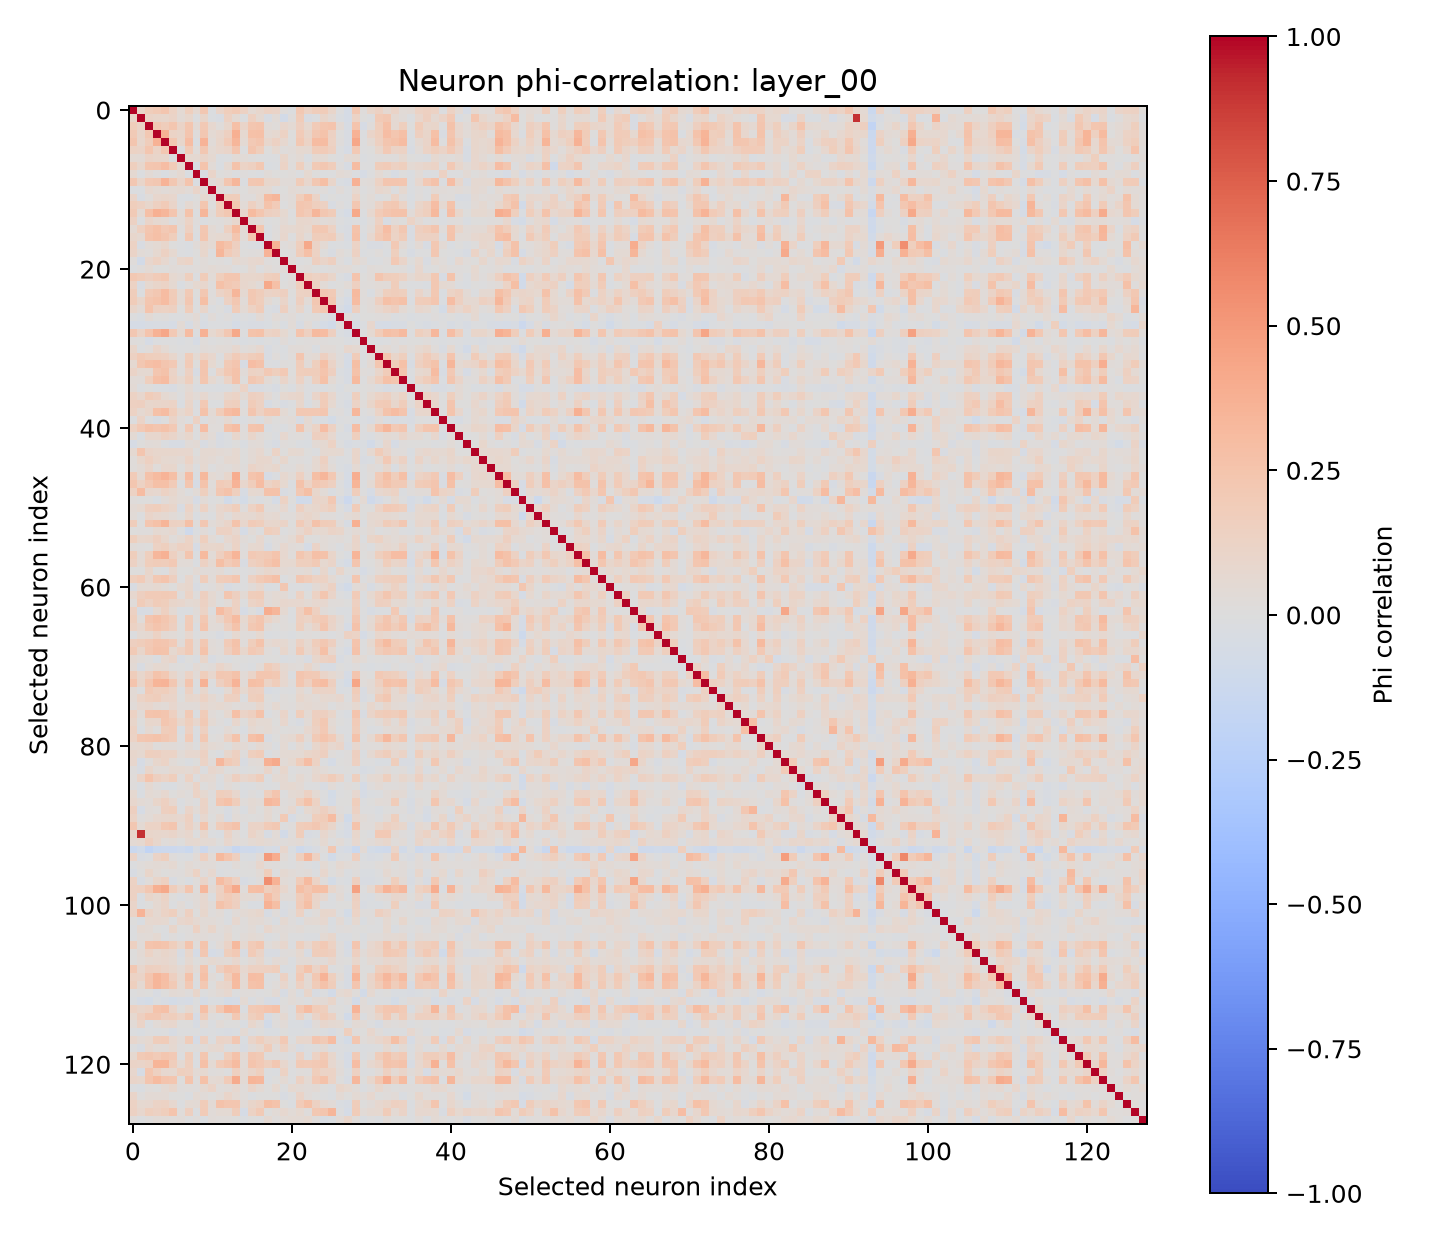
\includegraphics[width=\linewidth,height=3.6cm,keepaspectratio]{assets/rq2_coactivation.png}
\vspace{1pt}
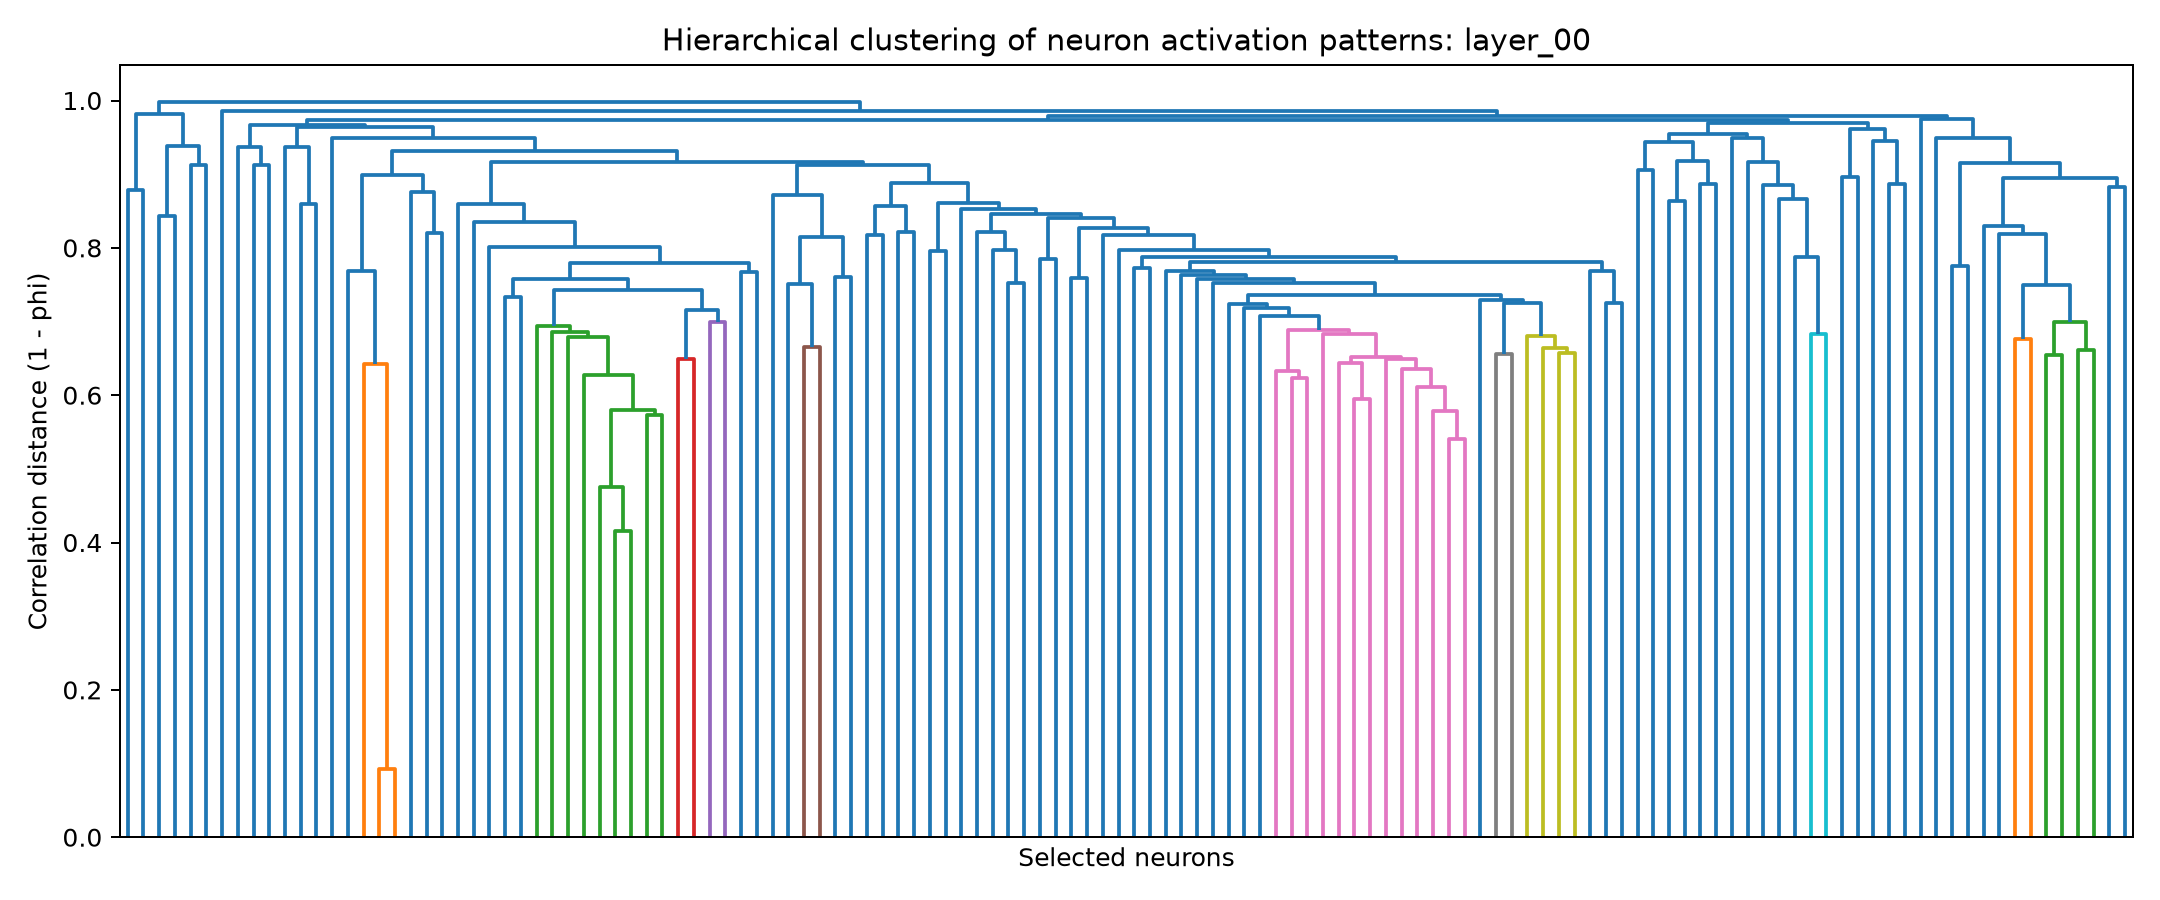
\includegraphics[width=\linewidth,height=1.25cm,keepaspectratio]{assets/rq2_dendrogram.png}
\column{.36\textwidth}
\begin{block}{Layer 0: coordinated firing}
\Large\color{ForestTeal}\bfseries 76.82\%\par
\small positive pairs; mean $\phi=+0.0685$.
\end{block}
\begin{block}{Layer 6: near-zero dependence}
\Large\color{ForestTeal}\bfseries $-0.0047$\par
\small median $\phi$; 45.14\% of pairs positive.
\end{block}
\begin{block}{HAC structure}
\Large\color{ForestTeal}\bfseries 122 / 128\par
\small distinct clusters at distance threshold 0.70.
\end{block}
\end{columns}
\vspace{1pt}
\smallnote{The report gives Layer 6 median $\phi=-0.0047$; a previous supplied summary used $-0.009$.}
\end{frame}

% -----------------------------------------------------------------------------
% 12. RQ3 methods
% -----------------------------------------------------------------------------
\begin{frame}{RQ3 | Target and Mathematical Formulation}
\rqbadge{RQ3}\quad\textbf{Latent space structure and intrinsic dimensionality}
\begin{block}{Target}
Quantify how many orthogonal directions carry meaningful activation variation, without relying only on an arbitrary 80\% or 95\% variance cutoff.
\end{block}
\small
\begin{columns}[T,onlytextwidth]
\column{.49\textwidth}
\begin{block}{Covariance PCA and Participation Ratio}
For centred activation matrix $X$, let $S$ have eigenvalues $\lambda_1,\ldots,\lambda_m$:
\[
\PR(S)=\frac{[\operatorname{tr}(S)]^2}{\|S\|_F^2}
=\frac{(\sum_i\lambda_i)^2}{\sum_i\lambda_i^2}.
\]
\end{block}
\column{.49\textwidth}
\begin{block}{Roy--Vetterli entropy effective rank}
\[
p_i=\frac{\lambda_i}{\sum_j\lambda_j},
\qquad H=-\sum_i p_i\ln p_i,
\]
\[
\erank(S)=\exp(H).
\]
\end{block}
\end{columns}
\vspace{3pt}
\small\textbf{Split-half stability:}\quad
$\bar\rho_K=\dfrac{1}{K}\sum_{i=1}^{K}\sigma_i(V_A^T V_B)$,
where $\sigma_i$ are singular values of the cross-subspace projection.
\end{frame}

% -----------------------------------------------------------------------------
% 13. RQ3 results
% -----------------------------------------------------------------------------
\begin{frame}{RQ3 | Evidence: Severe Early Collapse, Mid-layer Expansion}
\begin{columns}[T,onlytextwidth]
\column{.52\textwidth}
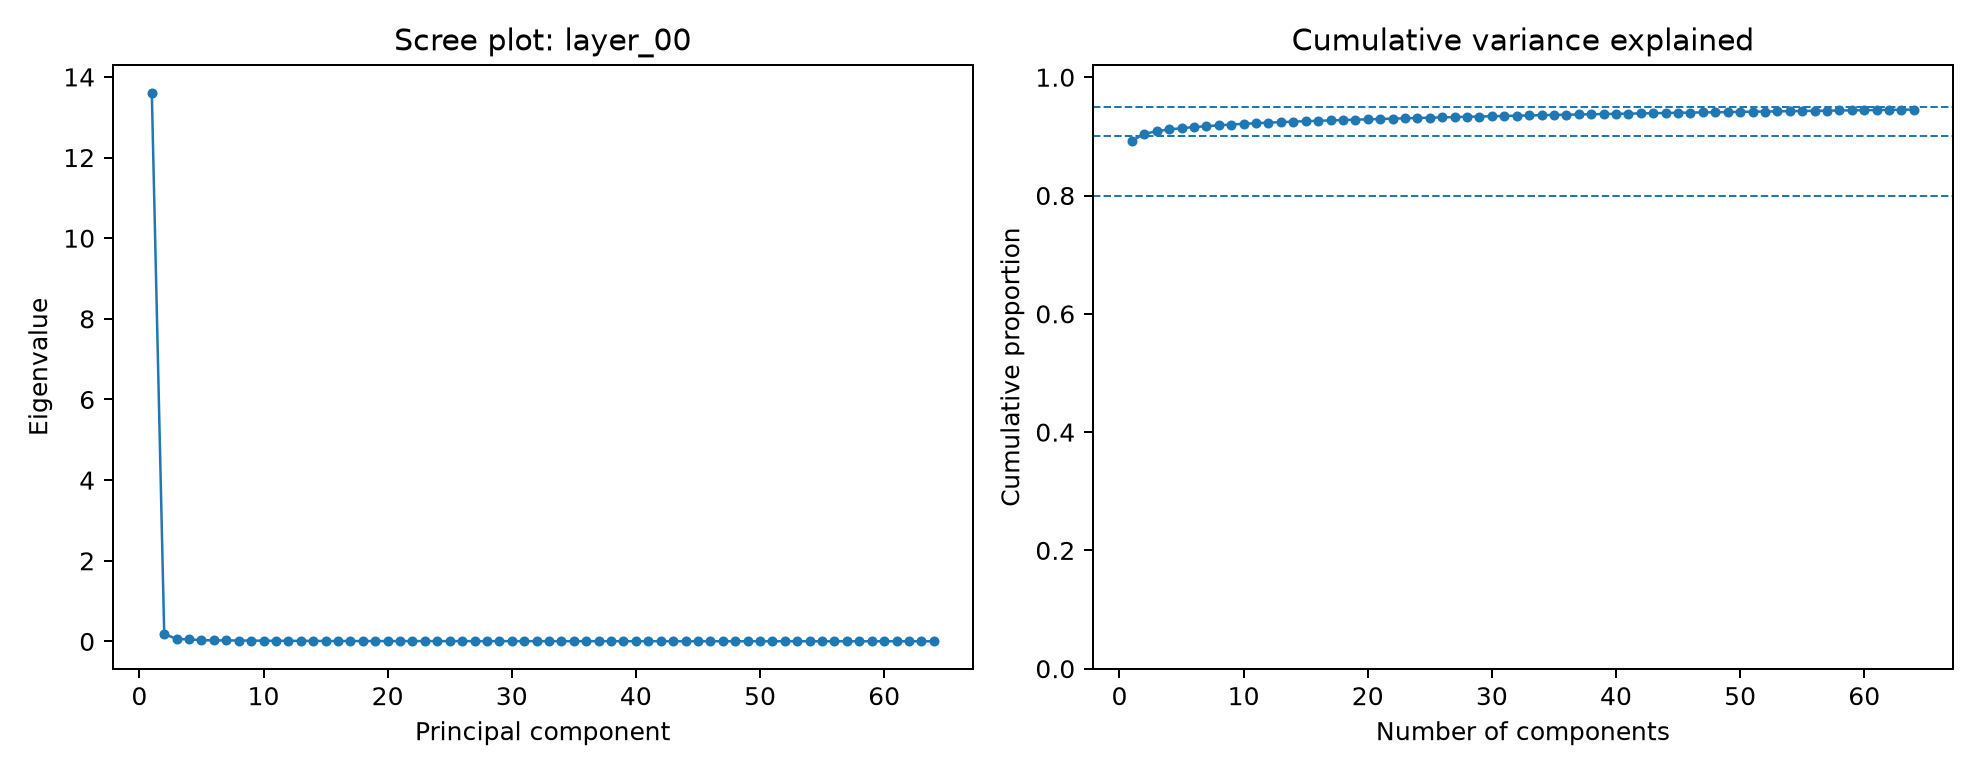
\includegraphics[width=\linewidth,height=3.9cm,keepaspectratio]{assets/rq3_pca.png}
\vspace{2pt}
\begin{block}{Layer 0}
\large\color{ForestTeal}\bfseries 81.4\%\par
\small variance explained by PC1.
\end{block}
\column{.46\textwidth}
\scriptsize
\begin{tabular}{lrrr}
\toprule
Layer & PR & erank & Stability $K=5$\\
\midrule
L0 & 1.12 & 1.51 & 0.894\\
L1 & 3.89 & 13.06 & 0.963\\
L2 & 1.20 & 1.86 & 0.986\\
L3 & 2.45 & 7.72 & 0.972\\
L4 & 3.51 & 12.19 & 0.977\\
L5 & 31.40 & 46.36 & 0.948\\
L6 & 29.86 & 45.53 & 0.964\\
L7 & 30.99 & 45.98 & 0.869\\
L8 & 31.42 & 46.10 & 0.976\\
L9 & 29.64 & 44.03 & 0.984\\
L10 & 27.64 & 41.43 & 0.971\\
L11 & 3.38 & 10.81 & 0.986\\
\bottomrule
\end{tabular}
\end{columns}
\vspace{3pt}
\small\textbf{Key distinction:} Layer 0 has $\PR=1.12$ and entropy effective rank $\erank=1.51$; these are different measures. Middle-layer entropy rank reaches about 41--46.
\end{frame}

% -----------------------------------------------------------------------------
% 14. RQ4 methods
% -----------------------------------------------------------------------------
\begin{frame}{RQ4 | Target and Mathematical Formulation}
\rqbadge{RQ4}\quad\textbf{Static weight rank versus dynamic activation rank}
\begin{block}{Target}
Test whether dense FFN weight matrices' spectral capacity is a reliable proxy for the effective dimensionality of token activations.
\end{block}
\small
\begin{columns}[T,onlytextwidth]
\column{.49\textwidth}
\begin{block}{Singular Value Decomposition}
For each projection matrix:
\[
W=U\Sigma V^T,\qquad
\Sigma=\operatorname{diag}(\sigma_1,\ldots,\sigma_{768}).
\]
\[
p_{i,W}=\frac{\sigma_i^2}{\sum_j\sigma_j^2}.
\]
\end{block}
\column{.49\textwidth}
\begin{block}{Compare layer-wise dimensions}
\[
\erank_W=\exp\!\left(-\sum_i p_{i,W}\ln p_{i,W}\right),
\]
\[
\erank_A=\exp\!\left(-\sum_i p_{i,A}\ln p_{i,A}\right).
\]
Estimate Pearson $r$ and Spearman $\rho$ across 12 layers.
\end{block}
\end{columns}
\vspace{2pt}
\smallnote{OPT-125M matrices: fc1/up-projection $3072\times768$; fc2/down-projection $768\times3072$. Each has at most 768 singular values.}
\end{frame}

% -----------------------------------------------------------------------------
% 15. RQ4 results
% -----------------------------------------------------------------------------
\begin{frame}{RQ4 | Evidence: Weight Capacity and Activation Geometry Decouple}
\begin{columns}[T,onlytextwidth]
\column{.57\textwidth}
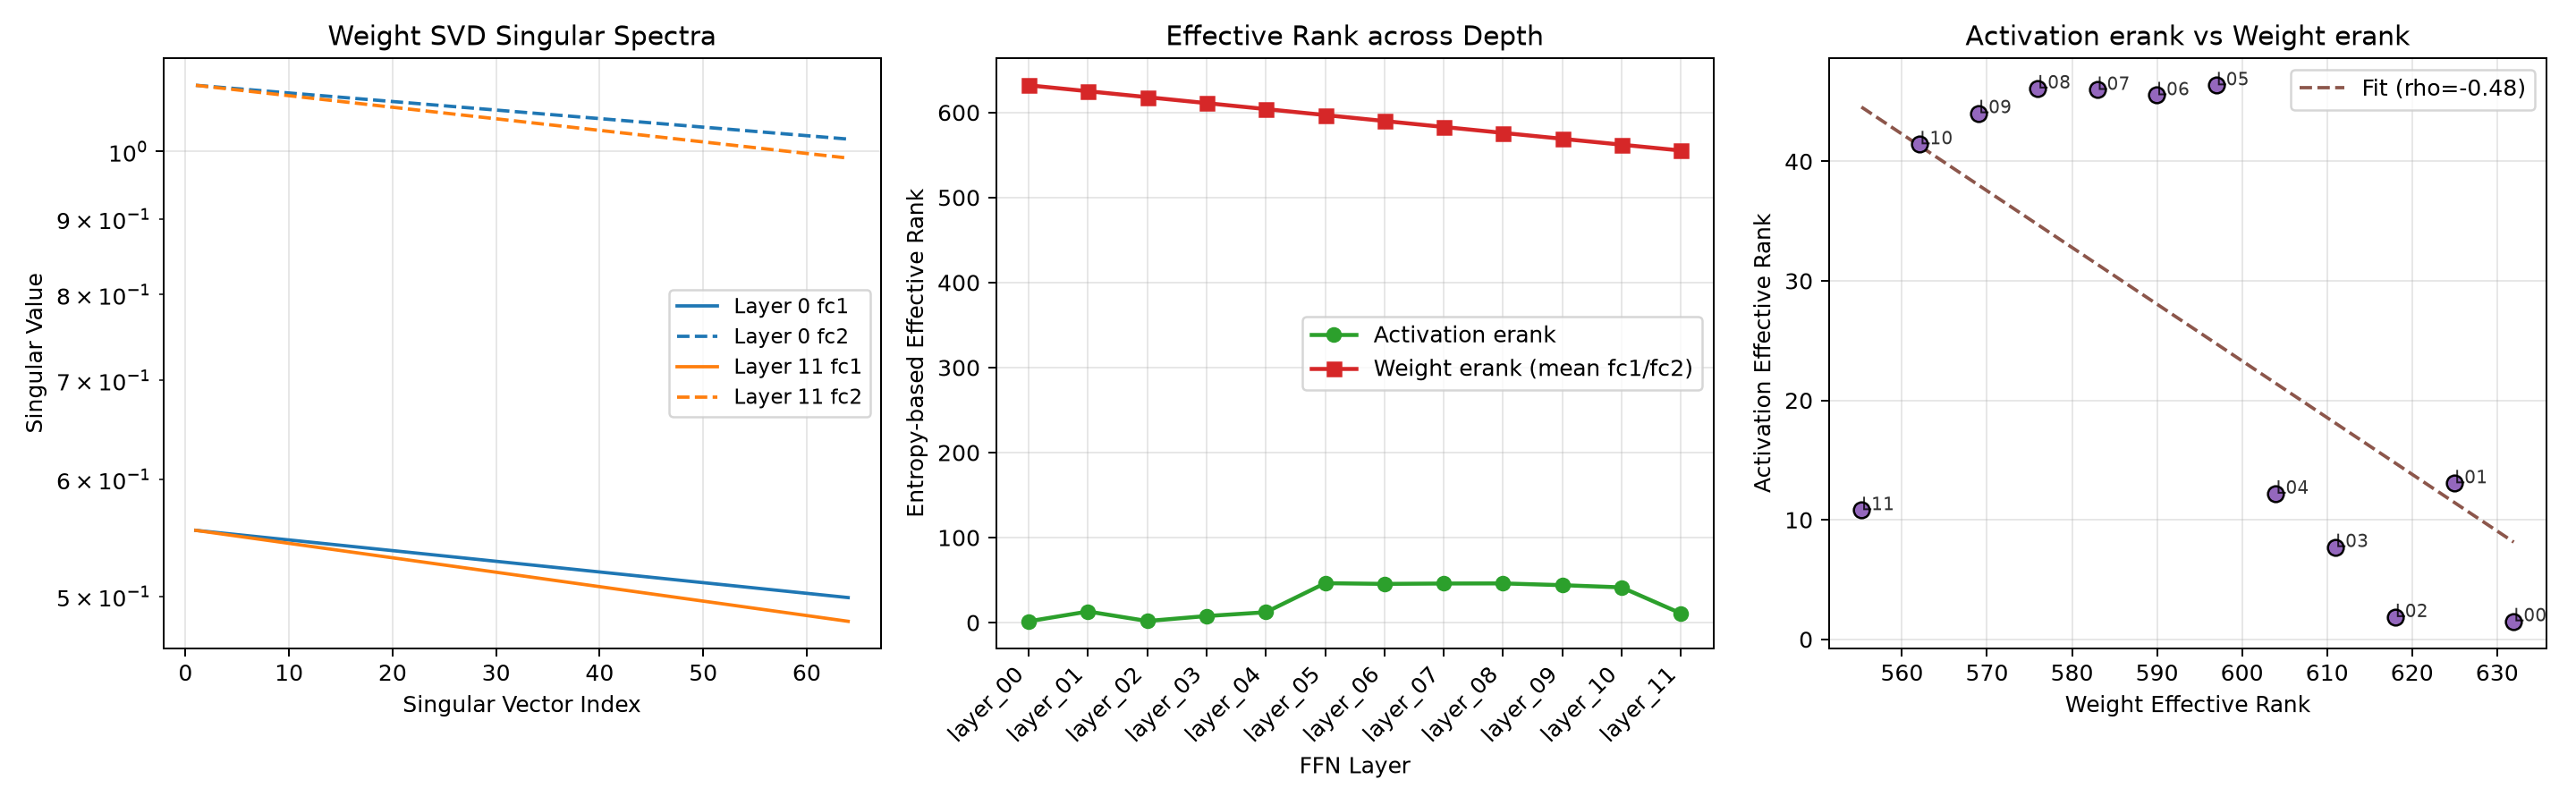
\includegraphics[width=\linewidth,height=3.25cm,keepaspectratio]{assets/rq4_weight_activation.png}
\column{.41\textwidth}
\begin{block}{Effective-rank comparison}
\small
\textbf{Mean weight rank:} $\erank_W=593.51$ (maximum 768).\par\vspace{5pt}
\textbf{Mean activation rank:} $\erank_A=26.38$ (nominal dimension 3,072).\par\vspace{5pt}
\textbf{Mean rank-scale gap:} approximately $22.5\times$.
\end{block}
\end{columns}
\vspace{2pt}
\scriptsize
\begin{tabularx}{\linewidth}{X r r}
\toprule
Association & Coefficient & $p$-value\\
\midrule
Pearson, entropy effective rank & $r=-0.607$ & 0.036\\
Spearman, entropy effective rank & $\rho=-0.476$ & 0.118\\
Pearson, participation ratio & $r=-0.592$ & 0.042\\
Spearman, participation ratio & $\rho=-0.497$ & 0.101\\
\bottomrule
\end{tabularx}
\vspace{2pt}
\smallnote{Pearson associations are significant at 5\%; Spearman associations are negative but not significant at 5\%.}
\end{frame}

% -----------------------------------------------------------------------------
% 16. RQ5 methods
% -----------------------------------------------------------------------------
\begin{frame}{RQ5 | Target and Mathematical Formulation}
\rqbadge{RQ5}\quad\textbf{Cross-domain mean and covariance differences}
\begin{block}{Target and null hypothesis}
Test whether FFN activation representations are statistically invariant across Wikipedia, Scientific and News text:
\[
\Hnull:\boldsymbol\mu_{wiki}=\boldsymbol\mu_{sci}=\boldsymbol\mu_{news}.
\]
\end{block}
\small
\begin{columns}[T,onlytextwidth]
\column{.50\textwidth}
\begin{block}{MANOVA decomposition}
\[
T=H+E,
\]
\[
H=\sum_{g=1}^{G}n_g(\bar x_g-\bar x)(\bar x_g-\bar x)^T,
\]
\[
E=\sum_{g=1}^{G}\sum_{i=1}^{n_g}(x_{gi}-\bar x_g)(x_{gi}-\bar x_g)^T.
\]
\end{block}
\column{.47\textwidth}
\begin{block}{Wilks' Lambda and Pillai's Trace}
For eigenvalues $\xi_i$ of $E^{-1}H$:
\[
\Lambda=\prod_i\frac{1}{1+\xi_i}
=\frac{\det(E)}{\det(H+E)},
\]
\[
V=\sum_i\frac{\xi_i}{1+\xi_i}.
\]
\end{block}
\end{columns}
\vspace{2pt}
\smallnote{Box's $M$ tests $H_0:\Sigma_1=\Sigma_2=\Sigma_3$; LDA evaluates how well projected activation coordinates discriminate domain labels.}
\end{frame}

% -----------------------------------------------------------------------------
% 17. RQ5 results
% -----------------------------------------------------------------------------
\begin{frame}{RQ5 | Evidence: Activation Manifolds Encode Text Domain}
\begin{columns}[T,onlytextwidth]
\column{.54\textwidth}
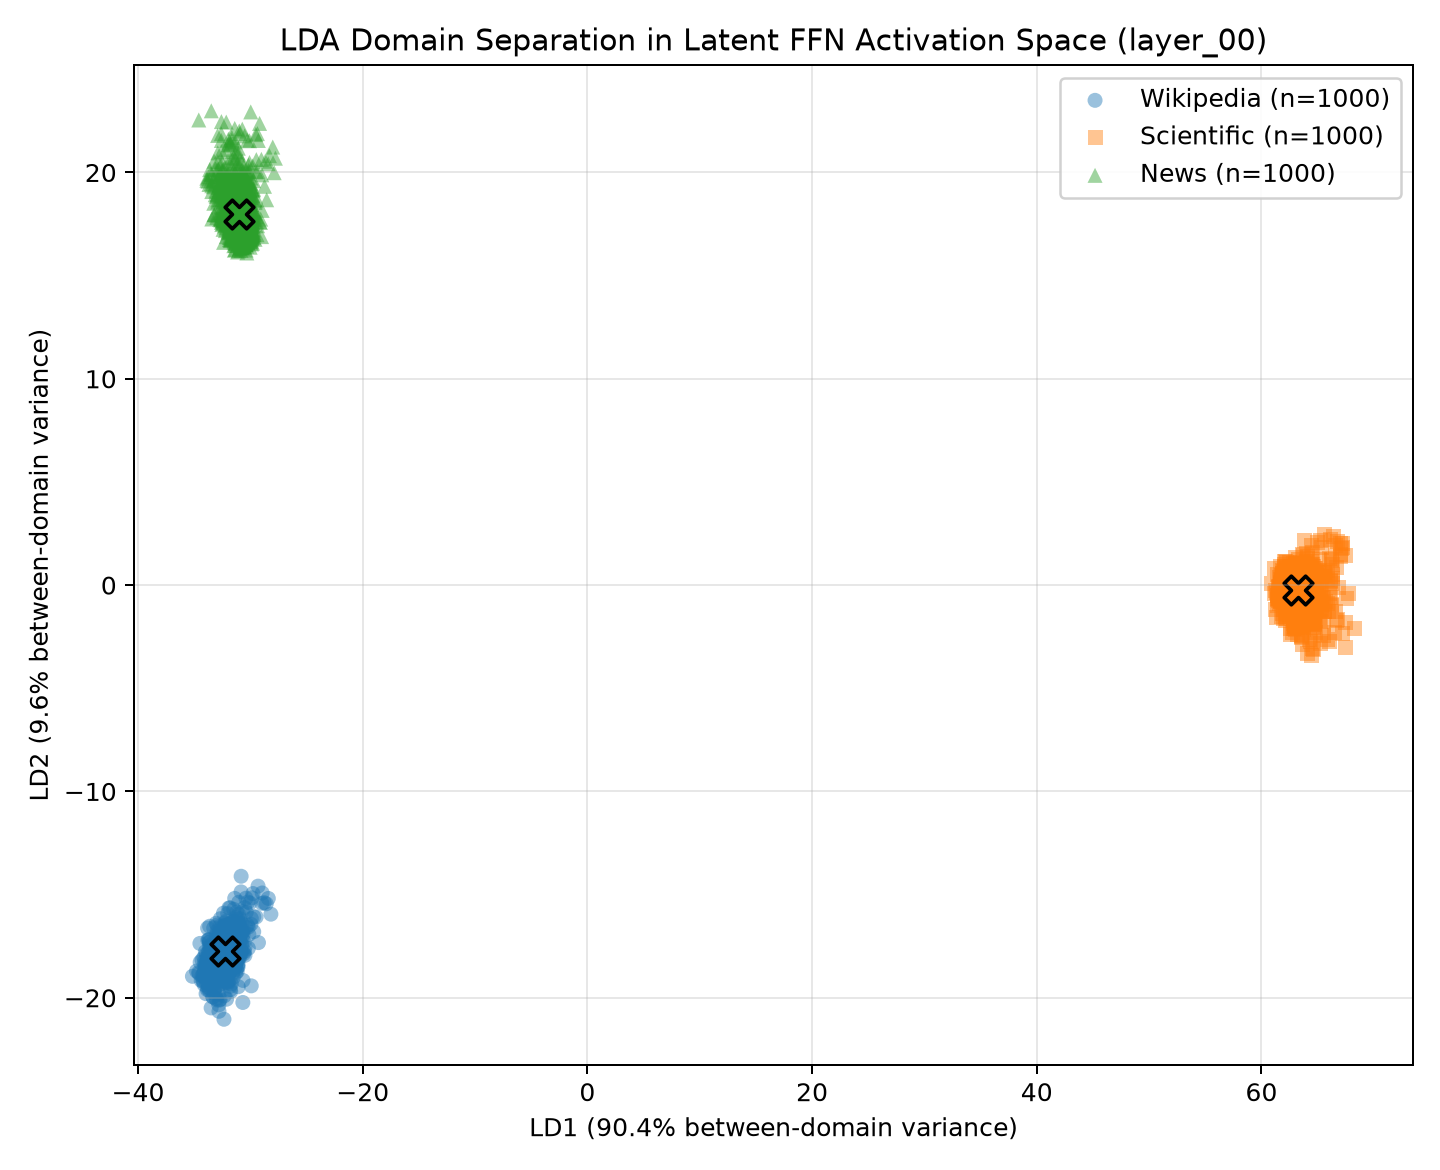
\includegraphics[width=\linewidth,height=3.1cm,keepaspectratio]{assets/rq5_lda.png}
\column{.44\textwidth}
\begin{block}{Key domain-separation results}
\small
\textbf{Wilks' Lambda:} $2.33\times10^{-6}$.\par\vspace{4pt}
\textbf{Pillai's Trace:} 1.995.\par\vspace{4pt}
\textbf{5-fold CV LDA accuracy:} 100\% (three-class chance baseline: 33.3\%).
\end{block}
\end{columns}
\vspace{2pt}
\tiny
\begin{tabularx}{\linewidth}{X l l}
\toprule
Test / metric & Reported result & Decision\\
\midrule
One-way MANOVA & Rao $F(16,5980)=244,389.3$ & Reject $\Hnull$\\
Box's $M$ & $M=15,693.7$; $\chi^2(72)=15,635.1$ & Reject covariance equality\\
Pairwise Hotelling & All pairs: $T^2>5.9\times10^5$ & Reject pairwise equality\\
5-fold CV LDA & 100.0\%; SD = 0.00 & Domains discriminable\\
\bottomrule
\end{tabularx}
\vspace{2pt}
\smallnote{The report prints $p=0.0$ for multivariate tests (numerical output precision); this is not a probability exactly equal to zero. Domain-aware routing is a proposed application, not an implemented system.}
\end{frame}

% -----------------------------------------------------------------------------
% 18. Master synthesis matrix
% -----------------------------------------------------------------------------
\begin{frame}{Master Summary Matrix: What the Five RQs Establish}
\scriptsize
\begin{tabularx}{\linewidth}{>{\bfseries}p{0.055\linewidth} p{0.19\linewidth} p{0.32\linewidth} X}
\toprule
RQ & Target & Key empirical evidence & Architectural conclusion\\
\midrule
RQ1 & Sparsity flatness & Layer 3 = 98.77\%; GG $p=1.68\times10^{-46}$; Friedman $p=5.99\times10^{-86}$ & Sparsity changes with depth; one threshold for every layer is not supported.\\[4pt]
RQ2 & Neuron independence & Layer 0 mean $\phi=+0.0685$; Layer 6 median $\phi=-0.0047$; 122/128 clusters at threshold 0.70 & Early co-activation structure weakens substantially with depth.\\[4pt]
RQ3 & Full-rank latent space & Layer 0 PR = 1.12, erank = 1.51; Layers 5--10 erank $\approx41$--46; split-half stability 0.869--0.986 & Activations occupy a compact, repeatable subspace rather than all 3,072 dimensions.\\[4pt]
RQ4 & Weight/activation coupling & Mean $\erank_W=593.51$ vs $\erank_A=26.38$; Pearson $r=-0.607$, $p=0.036$ & Static weight spectrum is not a direct proxy for dynamic activation rank.\\[4pt]
RQ5 & Domain invariance & Wilks $\Lambda=2.33\times10^{-6}$; Box's $M=15,693.7$; LDA = 100\% & Activation distributions carry strong domain-specific statistical signatures.\\
\bottomrule
\end{tabularx}
\vspace{7pt}
\takeaway{Across all five questions, the common pattern is structured sparsity: it varies by layer, by neuron pair, by latent direction and by text domain.}
\end{frame}

% -----------------------------------------------------------------------------
% 19. Architecture interpretation
% -----------------------------------------------------------------------------
\begin{frame}{Architectural Interpretation Across Network Depth}
\centering
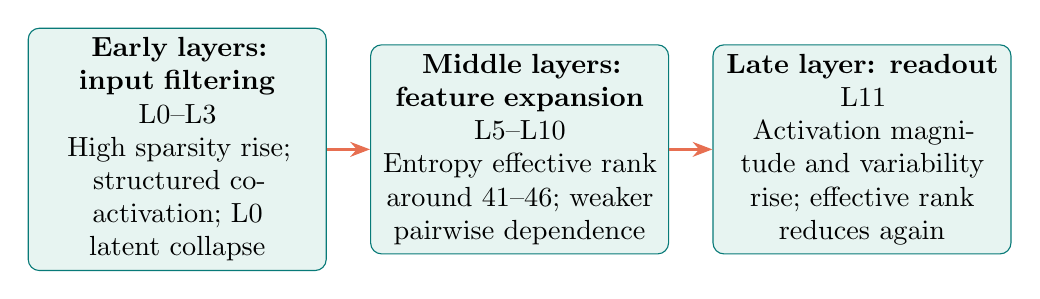
\begin{tikzpicture}[
  phase/.style={rounded corners=4pt,draw=ForestTeal,fill=TealTint,minimum height=1.5cm,text width=3.55cm,align=center},
  arr/.style={-{Stealth[length=2.5mm]},very thick,color=Coral}
]
\node[phase] (early) {\textbf{Early layers: input filtering}\\L0--L3\\High sparsity rise; structured co-activation; L0 latent collapse};
\node[phase,right=0.55cm of early] (middle) {\textbf{Middle layers: feature expansion}\\L5--L10\\Entropy effective rank around 41--46; weaker pairwise dependence};
\node[phase,right=0.55cm of middle] (late) {\textbf{Late layer: readout}\\L11\\Activation magnitude and variability rise; effective rank reduces again};
\draw[arr] (early)--(middle); \draw[arr] (middle)--(late);
\end{tikzpicture}
\vspace{0.65cm}
\begin{columns}[T,onlytextwidth]
\column{.32\textwidth}
\begin{block}{Layer profile}
Sparsity is non-flat; the strongest observed peak occurs at Layer 3.
\end{block}
\column{.32\textwidth}
\begin{block}{Neuron structure}
Co-activation clusters are clearer in Layer 0 than in Layer 6.
\end{block}
\column{.32\textwidth}
\begin{block}{Latent geometry}
Rank expands in middle layers and is not determined by weight rank alone.
\end{block}
\end{columns}
\smallnote{This slide summarises empirical patterns; it does not claim that the project directly proves the causal semantic role of any individual layer.}
\end{frame}

% -----------------------------------------------------------------------------
% 20. Engineering implications
% -----------------------------------------------------------------------------
\begin{frame}{Engineering Implications and Research Opportunities}
\begin{columns}[T,onlytextwidth]
\column{.49\textwidth}
\begin{block}{Supported by the results}
\begin{itemize}
  \item Explore layer-adaptive rather than uniform sparsity policies.
  \item Evaluate sparse kernels where zero fractions are high.
  \item Investigate low-rank approximations for layers with compact activation geometry.
  \item Avoid using static weight rank as a stand-alone proxy for activation rank.
\end{itemize}
\end{block}
\column{.48\textwidth}
\begin{alertblock}{Promising extensions (not implemented here)}
\begin{itemize}
  \item Domain-conditioned routing using learned activation features.
  \item Specialist FFN experts for scientific, news and encyclopedic text.
  \item Hardware-level profiling of sparse/low-rank execution.
  \item Accuracy-preserving pruning and reconstruction ablations.
\end{itemize}
\end{alertblock}
\end{columns}
\takeaway{The statistics motivate targeted compression and conditional computation experiments. Any claim of zero accuracy loss or measured speed-up requires a separate intervention study.}
\end{frame}

% -----------------------------------------------------------------------------
% 21. Limitations and future work
% -----------------------------------------------------------------------------
\begin{frame}{Limitations and Future Work}
\begin{columns}[T,onlytextwidth]
\column{.48\textwidth}
\begin{block}{Current limitations}
\begin{itemize}
  \item One frozen model: OPT-125M.
  \item Primary sparsity analysis uses WikiText-2.
  \item ReLU gives exact zeros; results do not automatically transfer to GELU or SwiGLU.
  \item Domain tests use a reduced $K=8$ PCA space for stable covariance estimation.
  \item Rank and co-activation statistics are observational, not causal tests.
\end{itemize}
\end{block}
\column{.49\textwidth}
\begin{exampleblock}{Future directions}
\begin{itemize}
  \item Scale to larger Transformer models and diverse benchmarks.
  \item Compare ReLU, GELU and SwiGLU activation families.
  \item Test pruning and low-rank reconstruction with held-out perplexity.
  \item Evaluate sparse inference on real hardware.
  \item Study runtime domain-aware routing and its overhead.
\end{itemize}
\end{exampleblock}
\end{columns}
\end{frame}

% -----------------------------------------------------------------------------
% 22. Conclusion
% -----------------------------------------------------------------------------
\begin{frame}{Conclusion}
\begin{block}{What this project contributes}
A multivariate statistical characterisation of post-ReLU FFN activations across all 12 layers of OPT-125M, combining profile analysis, binary dependence, PCA/effective rank, weight SVD and cross-domain MANOVA/LDA.
\end{block}
\begin{enumerate}
  \item Sparsity is strongly depth-dependent, with a 98.77\% peak at Layer 3.
  \item Early-layer neuron co-activation becomes much weaker by Layer 6.
  \item Activation variation is concentrated in a compact latent subspace.
  \item Dense weight matrices remain high-rank while dynamic activations are low-rank.
  \item FFN activation distributions strongly discriminate between text domains.
\end{enumerate}
\takeaway{The key result is not simply that FFN activations are sparse: their sparsity, dependence and dimensionality are structured and vary systematically with both network depth and input domain.}
\end{frame}

% -----------------------------------------------------------------------------
% 23. Numerical reconciliation note (appendix)
% -----------------------------------------------------------------------------
\appendix
\begin{frame}{Appendix | Numerical Values to Reconcile Before Final Submission}
\small
The main slides use the values printed in the final project report (Chapter 4, Tables 4.1--4.5 and Appendix B). Some values in the separately supplied summary differ:
\vspace{3pt}
\scriptsize
\begin{tabularx}{\linewidth}{p{0.10\linewidth} X X}
\toprule
Area & Supplied summary / earlier deck & Final report values used in this LaTeX deck\\
\midrule
RQ1 RM-ANOVA & $F(11,209)=176.43$; GG df $(1.38,26.2)$ & $F=1,838.82$, df $(11,429)$; GG df $(1.38,53.7)$; $p_{GG}=1.68\times10^{-46}$\\
RQ2 Layer 6 & Median $\phi=-0.009$ & Median $\phi=-0.0047$; 45.14\% positive pairs\\
RQ3 Layer 0 & PR reported as 1.51 & PR = 1.12; entropy effective rank = 1.51\\
RQ4 rank / Spearman & $\erank_A=26.10$; $\rho=-0.622$, $p=0.031$ & $\erank_A=26.38$; $\rho=-0.476$, $p=0.118$\\
RQ5 MANOVA & $F(16,178)=153.21$; Pillai = 1.84 & Rao $F(16,5980)=244,389.3$; Pillai = 1.995\\
\bottomrule
\end{tabularx}
\vspace{5pt}
\begin{alertblock}{Please verify}
If the supplied values come from a newer experimental rerun, update the report and all tables consistently before the final defence. Do not mix test statistics from different runs or label entropy effective rank as Participation Ratio.
\end{alertblock}
\end{frame}

% -----------------------------------------------------------------------------
% 24. References and questions
% -----------------------------------------------------------------------------
\begin{frame}{References and Discussion}
\small
\begin{enumerate}
  \item M. Geva, R. Schuster, J. Berant and O. Levy, ``Transformer Feed-Forward Layers Are Key-Value Memories,'' EMNLP, 2021.
  \item Z. Li, C. Wang, Y. Gu, C. Liu and J. Chen, ``On Emergence of Activation Sparsity in Trained Transformers,'' ICLR, 2023.
  \item R. A. Johnson and D. W. Wichern, \emph{Applied Multivariate Statistical Analysis}, 6th ed., Pearson, 2014.
  \item O. Roy and M. Vetterli, ``The Effective Rank: A Measure of Effective Dimensionality,'' EUSIPCO, pp. 606--610, 2007.
  \item W. K. H\"ardle and L. Simar, \emph{Applied Multivariate Statistical Analysis}, Springer, 2019.
\end{enumerate}
\vspace{0.35cm}
\begin{center}
{\color{ForestTeal}\Huge\bfseries Thank You!}\\[5pt]
{\Large Questions and Discussion}\\[0.55cm]
{\normalsize Lakshmi Ganapathi Kodi (BT23MA005) \quad | \quad Saurabh Kumar Gupta (BT23MA006)}\\[3pt]
{\small Under the guidance of Prof. Ashis SenGupta}
\end{center}
\end{frame}

\end{document}
